\documentclass[aspectratio=166]{beamer}

\newif\ifwhite
\whitetrue
% %%%%%%%%%%%%%%%%%%%%%%%%%%%%%%%%%%%%%%%%%%%%%%%%%%%
% %%%%%%%%%%%%%%%%%%%%%%%%%%%%%%%%%%%%%%%%%%%%%%%%%%%
% PATH to the beamer-templates-v3 folder
\def\cspath{../../../../../../Latex-workspace/}
% %%%%%%%%%%%%%%%%%%%%%%%%%%%%%%%%%%%%%%%%%%%%%%%%%%%
% %%%%%%%%%%%%%%%%%%%%%%%%%%%%%%%%%%%%%%%%%%%%%%%%%%%
% Main declarations for this slides
\usepackage{\cspath beamer-templates-v3/theme}
\usetikzlibrary{shapes,arrows.meta}
\usetikzlibrary{arrows.meta}
\usetikzlibrary{shapes,snakes}
\usetikzlibrary{shapes}
\usetikzlibrary{decorations.pathreplacing}
\usetikzlibrary{arrows,automata,positioning}
\usetikzlibrary{shapes.symbols}
\usetikzlibrary{arrows.meta}
\usetikzlibrary{shapes,snakes}

\setbeamersize{text margin left=0cm}
\setbeamersize{text margin right=0cm}

\def\csminilogo{\cspath beamer-templates-v3/Figs/CentraleSupelec-Logo-V-color.png}
% %%%%%%%%%%%%%%%%%%%%%%%%%%%%%%%%%%%%%%%%%%%%%%%%%%%
% %%%%%%%%%%%%%%%%%%%%%%%%%%%%%%%%%%%%%%%%%%%%%%%%%%%
% The main document 
\begin{document}    
% %%%%%%%%%%%%%%%%%%%%%%%%%%%%%%%%%%%%%%%%%%%%%%%%%%%
% %%%%%%%%%%%%%%%%%%%%%%%%%%%%%%%%%%%%%%%%%%%%%%%%%%%
\begin{frame}[plain]

\centering
\scalebox{1.6}{
\begin{tikzpicture}[->,>=stealth,shorten >=1pt,auto,node distance=2.8cm, semithick]
\tikzstyle{every state}=[fill=red,draw=none,text=white]
  
\only<1>{\node[state] (A)                    {\bf s1};}
\only<2>{\node[state] (A)                    {\bf s1, I};}
\onslide<3->{\node[initial,state] (A)                    {\bf s1, I};}
\onslide<3->{\node[state]         (B) [right of=A] {\bf s2, I};}
\onslide<3->{\node[state]         (C) [right of=B] {\bf s3, I};}

\onslide<3->{
\path (A) edge     [bend left]         node {ev1} (B);
\path (B) edge     [bend left]         node {ev2} (C);}
\end{tikzpicture}
}

\end{frame}
% %%%%%%%%%%%%%%%%%%%%%%%%%%%%%%%%%%%%%%%%%%%%%%%%%%%
% %%%%%%%%%%%%%%%%%%%%%%%%%%%%%%%%%%%%%%%%%%%%%%%%%%% 
\end{document}
% %%%%%%%%%%%%%%%%%%%%%%%%%%%%%%%%%%%%%%%%%%%%%%%%%%%
% %%%%%%%%%%%%%%%%%%%%%%%%%%%%%%%%%%%%%%%%%%%%%%%%%%%
